\documentclass[12pt, letterpaper]{article}

\usepackage[english]{babel} % Sets the language and regional settings for English documents
\usepackage[utf8]{inputenc} % Allows the use of UTF-8 characters in the document
\usepackage[T1]{fontenc} % Specifies t\subsubsection*{Forma canónica reducida}
\usepackage[margin=2cm]{geometry} % Sets the page margins
\usepackage{makeidx} % Enables the creation of indexes
% \usepackage{natbib} % Provides flexible bibliography support
\usepackage{url} % Allows the use of URLs
\usepackage{enumitem} % Customizes the appearance of lists
\usepackage{listings} % Provides syntax highlighting for code listings
\usepackage[dvipsnames]{xcolor} % Allows the use of colors
\usepackage{parskip} % Modifies paragraph spacing
\usepackage{graphicx} % Enables the inclusion of graphics
\usepackage{tikz} % Allows the creation of graphics and diagrams
\usepackage{float}
\usepackage{hyperref} % Enables the creation of hyperlinks
\usepackage{amsmath} % Provides additional math environments and commands
\usepackage{circuitikz} % Allows the creation of electrical circuits
\usepackage{adjustbox} % Adjusts the size of the circuit diagrams
\usepackage{tcolorbox}
\usepackage{diagbox} % Allows the use of diagonal boxes in table cells
\usepackage{colortbl} % Allows coloring of table cells
\hypersetup{
    colorlinks=true,
    linkcolor=blue,
    urlcolor=blue
}
\usepackage{breakurl} % permite que los links se rompan en varias líneas
\definecolor{mygray}{gray}{0.9}

\usetikzlibrary{shapes.geometric, positioning}

\lstset{
	language=SQL,
	basicstyle=\ttfamily\small,
	keywordstyle=\color{blue},
	commentstyle=\color[rgb]{0,0.5,0},
	stringstyle=\color{red},
	numbers=left,
	numberstyle=\tiny\color{gray},
	stepnumber=1,
	numbersep=10pt,
	backgroundcolor=\color{white},
	showspaces=false,
	showstringspaces=false,
	breaklines=true,
	frame=single,
	tabsize=2, captionpos=b, lineskip=-1pt,
	extendedchars=true,
	literate={á}{{\'a}}1 {é}{{\'e}}1 {í}{{\'i}}1 {ó}{{\'o}}1 {ú}{{\'u}}1 {Á}{{\'A}}1 {É}{{\'E}}1 {Í}{{\'I}}1 {Ó}{{\'O}}1 {Ú}{{\'U}}1 {ñ}{{\~n}}1 {Ñ}{{\~N}}1 {¿}{{\textquestiondown}}1 {¡}{{\textexclamdown}}1
}

% VHDL language configuration
\lstdefinelanguage{VHDL}{
	morekeywords={entity, architecture, signal, port, in, out, inout, begin, end, process, if, then, else, elsif, case, when, others, for, while, loop, wait, library, use, std_logic, std_logic_vector, integer, boolean, rising_edge, falling_edge, component, generic, map, downto, to, and, or, not, xor, nand, nor, xnor},
	morecomment=[l]{--},
	morestring=[b]",
	sensitive=false,
	alsoletter={_}
}

% VHDL listings style
\lstdefinestyle{vhdl}{
	language=VHDL,
	basicstyle=\ttfamily\small,
	keywordstyle=\color{blue}\bfseries,
	commentstyle=\color[rgb]{0,0.6,0}\itshape,
	stringstyle=\color{red},
	numbers=left,
	numberstyle=\tiny\color{gray},
	stepnumber=1,
	numbersep=10pt,
	backgroundcolor=\color{white},
	showspaces=false,
	showstringspaces=false,
	breaklines=true,
	frame=single,
	tabsize=2,
	captionpos=b,
	lineskip=-1pt,
	extendedchars=true
}

\graphicspath{ {./img/} } % Sets the path for the graphics

\newlist{biblio}{enumerate}{1}
\setlist[biblio,1]{label=[\arabic*]}

\makeindex

\begin{document}

\begin{titlepage}

	\begin{tikzpicture}[remember picture,overlay]
		\node[anchor=north west, inner sep=30] at (current page.north west) {
			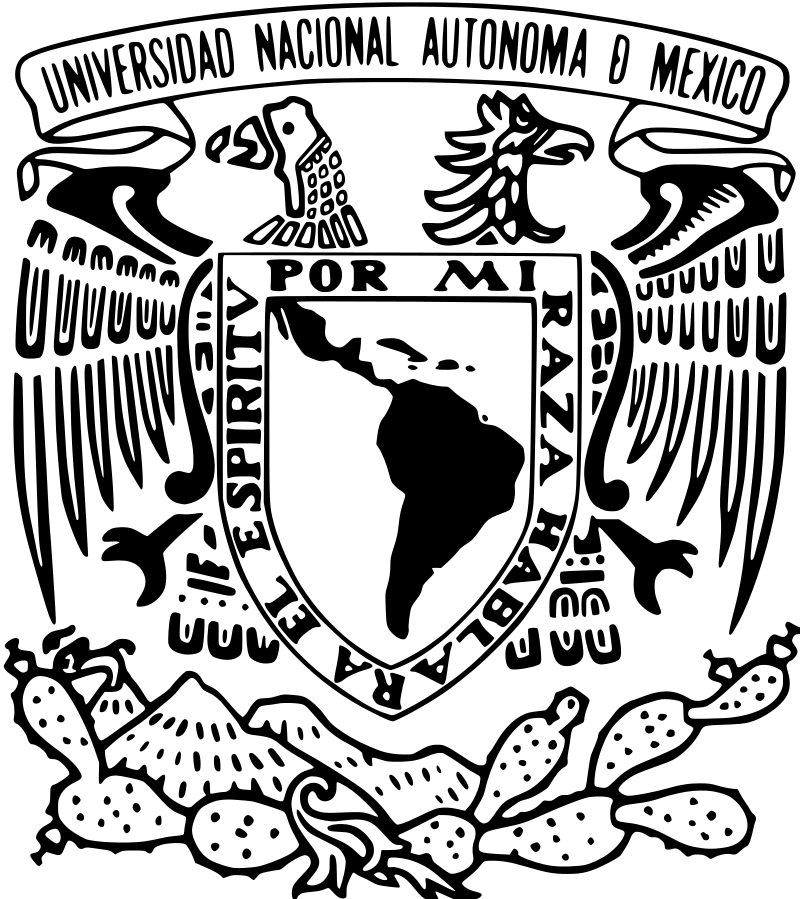
\includegraphics[width=4cm]{escudoUNAM.png}
		};

		\node[anchor=north east, inner sep=30] at (current page.north east) {
			
\includegraphics[width=4cm]{escudoFI.png}
		};
	\end{tikzpicture}

	\begin{center}
		\vspace*{3cm}

		\Huge
		\textbf{Previo 5 - Teorema de Redes}\\

		\vspace{2.5cm}

		\Huge
		\textbf{Facultad de Ingeniería}\\
		Circuitos Electrónicos\\
		\textbf{Ing. Martha Isela Torres Hernández} \\
		2026-1\\

		\vspace{2.5cm}

		\textbf{Grupo:} 4\\

		\vspace{2.5cm}

		\Huge
        \textbf{Integrantes Brigada 6:}\\
		Ugartechea González Luis Antonio\\
		Tepal Briseño Hansel Yael\\
		\textbf{Fecha de entrega:} 03 de noviembre del 2025\\
		\vspace{2.5cm}
	\end{center}
\end{titlepage}

\section{Determine los voltajes \(V_1\), \(V_2\), \(V_3\) y \(V_4\) del circuito de la figura \ref{fig:circuito1_1}; considere \(E \approx 12.0 V\)}

\begin{figure}[H]
	\centering
	
\includegraphics[width=0.6\textwidth]{circuito1_1.png}
	\caption{Circuito a analizar}
	\label{fig:circuito1_1}
\end{figure}

De acuerdo al circuito obtenemos el análisis de mallas y de nodos:

\begin{figure}[H]
	\centering
	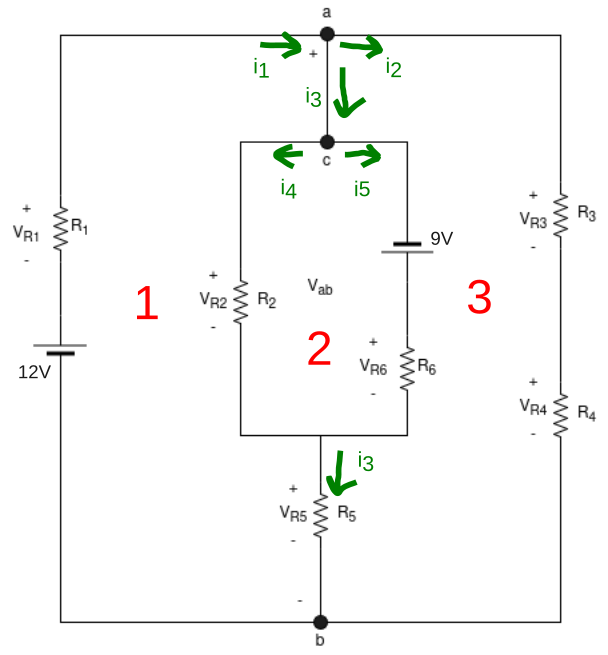
\includegraphics[width=0.5\textwidth]{circuito1_p1_edited.png}
	\caption{Circuito con mallas y nodos}
	\label{fig:circuito1_1}
\end{figure}

\textbf{De la malla 1 tenemos:}

\(E = V_{R_1} + V_{2} \Rightarrow V_{2} = E - V_{R_1}\)

Sustituyendo valores:

\begin{equation}
V_{2} = 12V - R_1(i_1)
\label{eq:eq1}
\end{equation}

\textbf{De la malla 2 tenemos:}

\(V_{R_2} = E_1 + V_{R_6}\)

Sustituyendo valores:

\(V_{R_2} = 9V + R_6(i_5)\)

Con esta ecuacion lo sumamos para obtener \(V_{2}\):

\(V_{2} = V_{R_2} + V_{R_5}\)

Tenemos que:

\begin{equation}
V_{2} = 9V + R_6(i_5) + R_5(i_3)
\label{eq:eq2}
\end{equation}

\begin{equation}
V_{2} = R_2(i_4) + R_5(i_3)
\label{eq:eq3}
\end{equation}

\textbf{De la malla 3 tenemos:}

\(V_{2} = V_{R_3} + V_{R_4}\)

Sustituyendo valores:

\begin{equation}
V_{2} = (i_2)(R_3 + R_4)
\label{eq:eq4}
\end{equation}

\textbf{Del nodo a tenemos:}

\begin{equation}
i_1 = i_2 + i_3
\label{eq:eq5}
\end{equation}

\textbf{Del nodo c tenemos:}

\begin{equation}
i_3 = i_4 + i_5
\label{eq:eq6}
\end{equation}

Con la ecuacion \ref{eq:eq5} despejamos \(i_3\):

\begin{equation}
i_3 = i_1 - i_2
\label{eq:eq7}
\end{equation}

Despejando \(i_1\) de la ecuacion \ref{eq:eq1} tenemos:

\(i_1 = \frac{12V - V_2}{R_1} = \frac{12V - V_2}{1000 \Omega}\)

Despejando \(i_2\) de la ecuacion \ref{eq:eq4} tenemos:

\(i_2 = \frac{V_2}{R_3+R_4} = \frac{V_2}{1000 \Omega + 10000 \Omega} = \frac{V_2}{11000 \Omega}\)

Sustituyendo \(i_1\) e \(i_2\) en la ecuacion \ref{eq:eq7}:

\begin{equation}
i_3 = \frac{12V - V_2}{1000 \Omega} - \frac{V_2}{11000 \Omega}
\label{eq:eq8}
\end{equation}

Despejando \(i_5\) de la ecuacion \ref{eq:eq2} tenemos:

\(i_5 = \frac{V_2 - 9V - R_5(i_3)}{R_6} = \frac{V_2 - 9V - 1000 \Omega (i_3)}{10000 \Omega}\)

Sustituyendo \(i_3\) de la ecuacion \ref{eq:eq8} en la ecuacion anterior:

\(i_5 = \frac{V_2 - 9V - 1000 \Omega \left( \frac{12V - V_2}{1000 \Omega} - \frac{V_2}{11000 \Omega} \right)}{10000 \Omega}\)

Desarrollando tenemos:

\(i_5 = \frac{-21V+\frac{V_2}{11}}{10000 \Omega}\)

\begin{equation}
i_5 = \frac{V_2}{110000 \Omega} - \frac{21V}{10000 \Omega}
\label{eq:eq9}
\end{equation}

Despejando \(i_4\) de la ecuacion \ref{eq:eq3} tenemos:

\(i_4 = \frac{V_2 - R_5(i_3)}{R_2} = \frac{V_2 - 1000 \Omega (i_3)}{10000 \Omega}\)

Sustituyendo \(i_3\) de la ecuacion \ref{eq:eq8} en la ecuacion anterior:

\(i_4 = \frac{V_2 - 1000 \Omega \left( \frac{12V - V_2}{1000 \Omega} - \frac{V_2}{11000 \Omega} \right)}{10000 \Omega}\)

Desarrollando tenemos:

\(i_4 = \frac{-12V + \frac{V_2}{11}}{10000 \Omega}\)

\begin{equation}
i_4 = \frac{V_2}{110000 \Omega} - \frac{12V}{10000 \Omega}
\label{eq:eq10}
\end{equation}

Sustituyendo \(i_3\), \(i_4\) y \(i_5\) en la ecuacion \ref{eq:eq6}:

\(\frac{12V - V_2}{1000 \Omega} - \frac{V_2}{11000 \Omega} = \frac{V_2}{110000 \Omega} - \frac{12V}{10000 \Omega} +\frac{V_2}{110000 \Omega} - \frac{21V}{10000 \Omega}\)

\(\frac{12V}{1000 \Omega} - \frac{V_2}{1000 \Omega} - \frac{V_2}{11000 \Omega} = \frac{V_2}{110000 \Omega} - \frac{12V}{10000 \Omega} +\frac{V_2}{110000 \Omega} - \frac{21V}{10000 \Omega}\)

\(12V - V_2 - \frac{V_2}{11} = \frac{V_2}{110} - 1.2V +\frac{V_2}{110} - 2.1V\)

\(- V_2 - \frac{V_2}{11} - \frac{V_2}{110} -\frac{V_2}{110} = - 1.2V - 2.1V - 12V \)

\(\frac{61}{55} \cdot V_2 = 15.3\)

Despejando \(V_2\):

\(V_2 = \frac{15.3(55)}{61}\)

\begin{tcolorbox}[colback=mygray, colframe=LimeGreen, boxrule=0.7pt, arc=2pt, boxsep=1pt, left=2pt, right=2pt, top=2pt, bottom=2pt, title=Resultado para \(V_2\)]
\[V_2 \approx 9 V\]
\end{tcolorbox}

Con \(V_2\) podemos calcular los demas voltajes:

Calculando \(V_1\):

\(V_1 = E - V_2 = 12V - 9V = 3V\)

\begin{tcolorbox}[colback=mygray, colframe=LimeGreen, boxrule=0.7pt, arc=2pt, boxsep=1pt, left=2pt, right=2pt, top=2pt, bottom=2pt, title=Resultado para \(V_1\)]
\[V_1 = 3 V\]
\end{tcolorbox}

Calculando \(V_3\):

\(V_2 = V_3 + V_4\)

Calculando la corriente \(i_2\):

\(i_2 = \frac{V_2}{R_3 + R_4} = \frac{9V}{1000 \Omega + 10000 \Omega} = \frac{9V}{11000 \Omega} = 0.00081818 A\)

Calculando \(V_3\):

\(V_3 = R_3(i_2) = 1000 \Omega (0.00081818 A) = 0.81818 V\)

\begin{tcolorbox}[colback=mygray, colframe=LimeGreen, boxrule=0.7pt, arc=2pt, boxsep=1pt, left=2pt, right=2pt, top=2pt, bottom=2pt, title=Resultado para \(V_3\)]
\[V_3 = 0.81818 V\]
\end{tcolorbox}

Calculando \(V_4\):

\(V_4 = R_4(i_2) = 10000 \Omega (0.00081818 A) = 8.1818 V\)

\begin{tcolorbox}[colback=mygray, colframe=LimeGreen, boxrule=0.7pt, arc=2pt, boxsep=1pt, left=2pt, right=2pt, top=2pt, bottom=2pt, title=Resultado para \(V_4\)]
\[V_4 = 8.1818 V\]
\end{tcolorbox}

\section{Determine los voltajes \(V_1\), \(V_2\), \(V_3\) y \(V_4\) del circuito de la figura \ref{fig:circuito1_2}}

\begin{figure}[H]
	\centering
	
\includegraphics[width=0.6\textwidth]{circuito1_2.png}
	\caption{Circuito a analizar}
	\label{fig:circuito1_2}
\end{figure}

De acuerdo con el circuito \ref{fig:circuito1_2}, vemos que la Batería de 9V está en paralelo con \(V_2\), por lo tanto:

\begin{tcolorbox}[colback=mygray, colframe=LimeGreen, boxrule=0.7pt, arc=2pt, boxsep=1pt, left=2pt, right=2pt, top=2pt, bottom=2pt, title=Resultado para \(V_2\)]
\[V_2 = 9 V\]
\end{tcolorbox}

De igual forma para \(V_1\):

Tenemos la batería en paralelo con \(Y\) y \(V_1\), por lo tanto:

\(9V = E - V_1\)

Sustituyendo \(E\):

\(9V = 12V - V_1\)

Despejando \(V_1\):

\(V_1 = 12V - 9V = 3V\)

\begin{tcolorbox}[colback=mygray, colframe=LimeGreen, boxrule=0.7pt, arc=2pt, boxsep=1pt, left=2pt, right=2pt, top=2pt, bottom=2pt, title=Resultado para \(V_1\)]
\[V_1 = 3 V\]
\end{tcolorbox}

Para \(V_3\) y \(V_4\) utilizamos el mismo principio ya que está en paralelo con la batería de 9V, por lo tanto:

\(9V = V_3 + V_4 = R_3(i) + R_4(i) = (R_3 + R_4)(i)\)

Despejando la corriente \(i\) y sustituyendo \(R_3\) y \(R_4\):

\(i = \frac{9V}{1000 + 10000}\)

\(i = \frac{9V}{11000 \Omega} = 0.00081818 A\)

Calculando \(V_3\):

\(V_3 = R_3(i) = 1000 \Omega (0.00081818 A) = 0.81818 V\)

\begin{tcolorbox}[colback=mygray, colframe=LimeGreen, boxrule=0.7pt, arc=2pt, boxsep=1pt, left=2pt, right=2pt, top=2pt, bottom=2pt, title=Resultado para \(V_3\)]
\[V_3 = 0.81818 V\]
\end{tcolorbox}

Calculando \(V_4\):

\(V_4 = R_4(i) = 10000 \Omega (0.00081818 A) = 8.1818 V\)
\begin{tcolorbox}[colback=mygray, colframe=LimeGreen, boxrule=0.7pt, arc=2pt, boxsep=1pt, left=2pt, right=2pt, top=2pt, bottom=2pt, title=Resultado para \(V_4\)]
\[V_4 = 8.1818 V\]
\end{tcolorbox}

\section{Determine los voltajes \(V_1\), \(V_2\), \(V_3\) y \(V_4\) del circuito de la figura \ref{fig:circuito1_3}}

\begin{figure}[H]
	\centering
	
\includegraphics[width=0.6\textwidth]{circuito1_3.png}
	\caption{Circuito a analizar}
	\label{fig:circuito1_3}
\end{figure}

Como vemos en el circuito \ref{fig:circuito1_3}, el voltaje \(V_2\) es el voltaje de la batería, por lo tanto:

\begin{tcolorbox}[colback=mygray, colframe=LimeGreen, boxrule=0.7pt, arc=2pt, boxsep=1pt, left=2pt, right=2pt, top=2pt, bottom=2pt, title=Resultado para \(V_2\)]
\[V_2 = 9 V\]
\end{tcolorbox}

Para \(V_1\) tenemos que:

\(V_1 + V_2 = E\)

Sustituyendo \(E\) y \(V_2\):

\(V_1 + 9V = 12V\)

Despejando \(V_1\):

\(V_1 = 12V - 9V = 3V\)

\begin{tcolorbox}[colback=mygray, colframe=LimeGreen, boxrule=0.7pt, arc=2pt, boxsep=1pt, left=2pt, right=2pt, top=2pt, bottom=2pt, title=Resultado para \(V_1\)]
\[V_1 = 3 V\]
\end{tcolorbox}

Para \(V_3\) y \(V_4\) utilizamos el mismo principio ya que está en paralelo con la batería de 9V, por lo tanto:

\(9V = V_3 + V_4 = R_3(i) + R_4(i) = (R_3 + R_4)(i)\)

Despejando la corriente \(i\) y sustituyendo \(R_3\) y \(R_4\):

\(i = \frac{9V}{1000 + 10000}\)

\(i = \frac{9V}{11000 \Omega} = 0.00081818 A\)

Calculando \(V_3\):

\(V_3 = R_3(i) = 1000 \Omega (0.00081818 A) = 0.81818 V\)

\begin{tcolorbox}[colback=mygray, colframe=LimeGreen, boxrule=0.7pt, arc=2pt, boxsep=1pt, left=2pt, right=2pt, top=2pt, bottom=2pt, title=Resultado para \(V_3\)]
\[V_3 = 0.81818 V\]
\end{tcolorbox}

Calculando \(V_4\):

\(V_4 = R_4(i) = 10000 \Omega (0.00081818 A) = 8.1818 V\)
\begin{tcolorbox}[colback=mygray, colframe=LimeGreen, boxrule=0.7pt, arc=2pt, boxsep=1pt, left=2pt, right=2pt, top=2pt, bottom=2pt, title=Resultado para \(V_4\)]
\[V_4 = 8.1818 V\]
\end{tcolorbox}

\section{¿Qué se puede concluir?}

Esto demuestra que podemos sustituir completamente una rama de un circuito por una batería de voltaje igual a la caída de voltaje en esa rama sin alterar el comportamiento del circuito en los demás nodos. Esto es útil para simplificar el análisis de circuitos complejos al reducir el número de componentes que deben considerarse directamente.

\section{Determine para el circuito para la figura \ref{fig:circuito2_1} la diferencia de potencial \(V_{ab}\)}

\begin{figure}[H]
	\centering
	
\includegraphics[width=0.6\textwidth]{circuito2_1.png}
	\caption{Circuito a analizar}
	\label{fig:circuito2_1}
\end{figure}

Utilizando Ley de corriente de Kirchhoff en el nodo \(a\):

\[I_1 + I_2 = I_3\]

utilizando ley de ohm para cada resistencia:

\[I_1 = \frac{V_a - 9 V}{1000 \Omega}\]

\[I_2 = \frac{V_a - 9 V}{1000 \Omega}\]

\[I_3 = \frac{Va - V_b}{10000 \Omega}\]

Suponiendo que el voltaje \(V_b = 0\)

\[\frac{V_a - 9 V}{1000 \Omega} + \frac{V_a - 9 V}{1000 \Omega} = \frac{V_a}{10000 \Omega}\]

Multiplicando por \(10000 \Omega\) para eliminar los denominadores:

\[10 (V_a - 9 V) + 10 (V_a - 9 V) = V_a\]

\[20 (V_a - 9 V) = V_a\]

\[21 V_a = 180 \]

\[V_a = 8.5714\]

\begin{tcolorbox}[colback=mygray, colframe=LimeGreen, boxrule=0.7pt, arc=2pt, boxsep=1pt, left=2pt, right=2pt, top=2pt, bottom=2pt, title=Resultado para \(V_{ab}\)]
\(V_{ab} = 8.5714 V\)
\end{tcolorbox}

\section{Determine para el circuito para la figura \ref{fig:circuito2_2} la diferencia de potencial \(V_{a'b'}\)}

\begin{figure}[H]
	\centering
	
\includegraphics[width=0.5\textwidth]{circuito2_2.png}
	\caption{Circuito a analizar}
	\label{fig:circuito2_2}
\end{figure}

Utilizando Divisor de voltaje, simplificamos la resistencia de lado izquierdo que esta en paralelo con la resistencia central:

\[R_{eq1} = \frac{1 k \Omega \cdot 10 k \Omega}{1 k \Omega + 10 k \Omega} = \frac{10 k \Omega}{11 k \Omega}\]

Encontrando la resistencia equivalente sumamos la resistencia obtenida con la que se encuntra en serie:

\[R_{eq} = 1 k \Omega + \frac{10 k \Omega}{11 k \Omega} = \frac{21}{11}\]

Utilizando la formula de divisor de voltaje tenemos:

\[V_{a'b'} = \frac{R_{eq1}}{R_{eq}} \cdot 9 V\]

\[V_{a'b'} = \frac{\frac{10}{11}K \Omega}{\frac{21}{11} k \Omega} \cdot 9 V\]

\[V_{a'b'} = \frac{10 k \Omega}{21 k \Omega} \cdot 9 V\]

\[V_{a'b'} = \frac{90}{21} V = 4.2857 V\]

\begin{tcolorbox}[colback=mygray, colframe=LimeGreen, boxrule=0.7pt, arc=2pt, boxsep=1pt, left=2pt, right=2pt, top=2pt, bottom=2pt, title=Resultado para \(V_{a'b'}\)]
\[V_{a'b'} = 4.2857 V\]
\end{tcolorbox}

\section{Determine para el circuito para la figura \ref{fig:circuito2_3} la diferencia de potencial \(V_{a''b''}\)}


\begin{figure}[H]
	\centering
	
\includegraphics[width=0.5\textwidth]{circuito2_3.png}
	\caption{Circuito a analizar}
	\label{fig:circuito2_3}
\end{figure}

Ya que este circuito es exactamente igual al inciso anterior, siendo la unica diferencia que la fuente cambia de ubicación. El cálculo para determinar la diferencia de potencia \(V_{a''b''}\) es exactamente el mismo por lo que:

\[V_{a''b''} = \frac{10 k \Omega}{21 k \Omega} \cdot 9 V\]

\[V_{a''b''} = \frac{90}{21} V = 4.2857 V\]

\begin{tcolorbox}[colback=mygray, colframe=LimeGreen, boxrule=0.7pt, arc=2pt, boxsep=1pt, left=2pt, right=2pt, top=2pt, bottom=2pt, title=Resultado para \(V_{a''b''}\)]
\[V_{a''b''} = 4.2857 V\]
\end{tcolorbox}

\section{Verifique con los resultados anteriores que \(V_{ab} = V_{a'b'} + V_{a''b''}\)}

Sabemos que:

\[
\begin{aligned}
V_{ab} &= 8.5714\ \mathrm{V} \\
V_{a'b'} &= 4.2857\ \mathrm{V} \\
V_{a''b''} &= 4.2857\ \mathrm{V}
\end{aligned}
\]

\[V_{ab} = V_{a'b'} + V_{a''b''}\]

\[8.5714\ \mathrm{V} = 4.2857\ \mathrm{V} + 4.2857\ \mathrm{V}\]

\begin{tcolorbox}[colback=mygray, colframe=LimeGreen, boxrule=0.7pt, arc=2pt, boxsep=1pt, left=2pt, right=2pt, top=2pt, bottom=2pt, title=Demostración de Superposición]
\[8.5714\ \mathrm{V} = 8.5714\ \mathrm{V}\]
\end{tcolorbox}

\textcolor{LimeGreen}{Por lo tanto queda demostrado.}

\section{Para el circuito de la figura \ref{fig:circuito3_1}, desarrolle las siguientes ecuaciones}

\[ \sum_{k=1}^{b} j_{k} V_{k} = \frac{1}{2} \sum_{\alpha=1}^{l+1} \sum_{\beta=1}^{l+1} (I_{\alpha} - I_{\beta}) V_{\alpha\beta} \]

\[ \sum_{k=1}^{b} j_{k} V_{k} = \frac{1}{2} \sum_{\alpha=1}^{l+1} I_{\alpha} \left( \sum_{\beta=1}^{l+1} V_{\alpha\beta} \right) - \frac{1}{2} \sum_{\beta=1}^{l+1} I_{\beta} \left( \sum_{\alpha=1}^{l+1} V_{\alpha\beta} \right) \]

\begin{figure}[H]
	\centering
	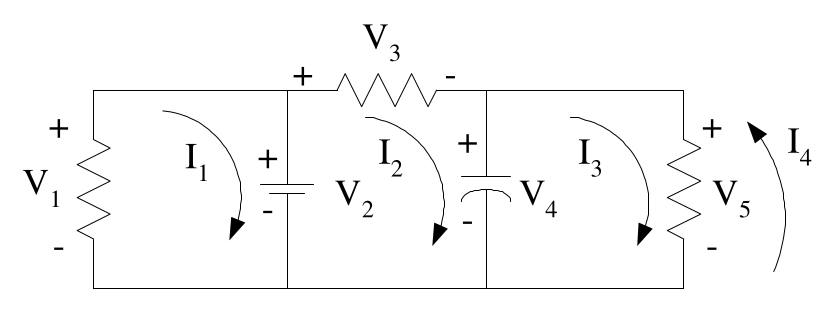
\includegraphics[width=0.6\textwidth]{circuito3_1.png}
	\caption{Circuito a analizar}
	\label{fig:circuito3_1}
\end{figure}

Para desarrollar las ecuaciones es necesario aplicar la ley de Kirchhoff de voltajes.

En la malla izquierda:

\[V_1 - V_2 = 0\]

En la malla central:

\[V_2 - V_3 - V_4 = 0\]

En la malla derecha:

\[V_4 - V_5 = 0\]

Ahora para calcular \( \sum_{k=1}^{b} j_{k} V_{k} \) debemos de calcular la potencia absorvida para cada componente. Por lo que utilizando las ecuaciones de las mallas tenemos:

\[ j_1 (V_1 - V_2) + j_2 (V_2 - V_3 - V_4) + j_3 (V_4 - V_5) = 0 \]

\[j_1 V_1 - j_1 V_2 + j_2 V_2 - j_2 V_3 - j_2 V_4 + j_3 V_4 - j_3 V_5 = 0\]

\[j_1 V_1 + V_2 (j_2 - j_1) - j_2 V_3 + V_4 (j_3 - j_2) - j_3 V_5 = 0\]

Por lo tanto tenemos que:

\begin{tcolorbox}[colback=mygray, colframe=LimeGreen, boxrule=0.7pt, arc=2pt, boxsep=1pt, left=2pt, right=2pt, top=2pt, bottom=2pt, title=Resultado de la ecuación desarrollada]
\[
\sum_{k=1}^{b} j_{k} V_{k} = j_1 V_1 + V_2 (j_2 - j_1) - j_2 V_3 + V_4 (j_3 - j_2) - j_3 V_5
\]
\end{tcolorbox}

% \begin{thebibliography}{9}
% \section{Bibliografía}
% \renewcommand{\refname}{}
%    \bibitem{} Dr. E. García, \textit{"Diseño Digital VLSI Repaso DDM"}, presentado en el curso de Diseño Digital VLSI, Ciudad de México, 2025.
% \end{thebibliography}

\end{document}
